\documentclass[11pt,dvipdfm]{article}
\usepackage{deauthor,times,graphicx}
%\graphicspath{{authorname/}} %for embedded figures
\begin{document} 
\title{Employing Blockchain Properties for Transparent Databases}
\author {Henry F. Korth\\ Lehigh University\\ blockchain.cse.lehigh.edu}
\maketitle
 \begin{abstract}
 Both transparency and privacy are important properties in most any
information-management application, yet they are in many ways inherently opposed to
each other.
The tradeoff between these two goals is typically intermediated by a trusted system or
organization.  The resulting tradeoff is  only as meaningful as the level of trust in the
intermediary.  
Blockchains provide a decentralized single source of truth that allows for the reduction or
elimination of the need for trust.
This paper explores the options in trading off transparency and privacy in a 
blockchain database.  
It also considers the closely-related concepts of accountability and auditability and explores
how cryptographic techniques  allow the disclosures needed for 
regulatable information systems while preserving
a high degree of privacy.

\end{abstract}
 
\section{Transparency Versus Privacy and the Role of Trust}
\label{hfk:hiding}
In a traditional enterprise information system, the database is the final source of truth.
The data in the database are closely guarded by access controls and 
integrity checking.
Privacy regulations often apply to the use of data (examples include the U.S.\
HIPPA and FERPA regulations for health and education records respectively).
Transparency regulations are exemplified by requirements that enterprises  provide financial statements
at specific intervals with specific content and by requirements that enterprises  disclose to each customer
what data they hold on that customer.
Despite these requirements, the entire process depends on a strong degree of trust in enterprises to
provide consistent and truthful disclosures.
Ensuring truthfulness requires an audit of enterprise data that, in turn, mandates further
disclosures at least to the auditors.
Increasing data disclosure can compromise privacy.

The blockchain properties of irrefutability, immutability, and anonymity \cite{DSC-BCDB}  offer useful tools in managing the tradeoffs among privacy, transparency, and trust.
However, much depends on how those tools are used.
A simple move to a blockchain database presents a variety of challenges.
A public blockchain is public to all.  The only secret is the mapping between blockchain IDs and
the identity of the corresponding real-world person or organization.  That mapping can often be
determined by correlation of on-chain and off-chain activity. 
The primary value of a blockchain in a transparent, privacy-preserving 
information system is its role as a trusted source of truth. The ``truth'' stored on that
blockchain  can take a variety of forms.  
From a database standpoint, the most important stored data are cryptographic commitments to protected data
(using Merkle trees \cite{Merkle87})  whose contents
can be disclosed in part or in aggregate with a proof of the correctness of such
disclosures.
In such a system, the blockchain holds mainly commitments.  Data themselves are stored off-chain
at much lower cost than on-chain storage.\footnote{On-chain storage costs vary.  On the Ethereum chain,
based on gas price and ETH prices at the time this paper was written, storing 1MB of data on-chain would
have cost about 30000 US dollars.  Decentralized storage services like Filecoin employ cryptographically-secured
off-chain storage.}

Disclosure of data is not the only trust consideration.  When the disclosure  is
some function computed over the actual full dataset, one must trust the agent who did the
computation.  A flawed computation from correct data is of no more use than inaccurate data.  Thus, beyond data, one must consider the provenance of data, that is, what data
were used in the computation and what code was used to do the computation.
Provenance in data has been studied at length for well over a decade \cite{margo}.
Zero-knowledge proofs\cite{micali} (henceforth, ZK-proofs) are a cryptographic method for allowing a
verifier to validate the correctness of an execution without having to know the actual data
on which the execution operated.  This makes it possible to prove that the disclosed result was 
produced by a specific program running on the same dataset to which a commitment was made.
No information need be revealed about the  data other than the result itself.
The combination of provenance management and ZK-proofs of execution enable transparent trust
not only in data but also in how those data were generated.

Our discussion of blockchain and database transparency is thus largely focused on trust.
The ability of a blockchain to move the focus of trust from centralized authorities to a decentralized
consensus creates trust in a process rather than in an opaque institution.
This re-focusing of trust can revolutionize virtually all information-driven applications.
A few examples follow:
\begin{itemize}
\item {\bf Supply chain: } Businesses enter into supply-chain agreements via a legally binding
contract.  Traditional day-to-day tracking of those relationships either depends on a trusted member of the
chain storing data or on a collection of separately managed  repositories.  A blockchain-based supply-chain
information system replaces that with cryptographic signatures\cite{dh76} for irrefutability,  and verifiable, distributed updates for immutability.
Trust in the final-product producer is limited only to that firm admitting the right set of users to the system.
The blockchain is a single source of supply information that enables fast, effective product recalls with no ``finger pointing'' among
suppliers trying to blame each other for supplying a defective component.
\item {\bf Real assets: } Governments maintain trusted records of asset ownership (real estate, vehicles, etc.).
These systems require trust not only in government but also in the controls implemented by government on
their databases.  Each transaction becomes a complex process of validation of identity -- of the parties involved and
of the asset involved.  In a blockchain-based system, the only function the government needs to provide is a
single, permanent mapping between the real asset and a unique blockchain token (that is, a non-fungible
token, or NFT\footnote{To be clear, our focus here is about assets like houses and cars, not cryptokitties,
cyberpunks,
bored apes, or something similar.}). Transactions regarding asset ownership then become simple blockchain
transactions requiring no central intermediation by government.
The amount of trust left to a central institution is limited to maintaining the physical-asset-to-NFT mapping.
\item {\bf Market making: } The creation of markets for trading stocks, exchanging currencies, etc.\ is a large, slow,
high-overhead business.  Most New York Stock Exchange trades take two business days to settle.
International funds transfer via the SWIFT system may be anything but what that name suggests.  The SWIFT 
system is a messaging system among correspondent banks, with funds transfers following the messaging.
The process can still take days.

In contrast, competing blockchain systems in this space take seconds (e.g., Stellar\cite{StellarSOSP19} and Ripple).
Automated market-makers  adjust prices with each trade.
Automated arbitrageurs maintain price-equivalence across markets.
No institution needs to be trusted; trust is in only publicly readable code.
\item {\bf Lending:}  Much like market-making, an automated system can manage real-time interest
rates both for lenders and borrowers.  Liquidators earn a fee for managing loans that become
under-collateralized and doing so in an automated manner.  
\end{itemize}
The list could go on. 
In each case, there is a gain in speed from taking humans out of the transaction path, and a gain in trustlessness
by removing or reducing the need to trust institutions whose operation is opaque.
Open-source security replaces institutional trust and ``security by obscurity.''

In what follows, we explore the implications of blockchain technology on traditional information-based applications
from the standpoints of transparency, privacy, and trust.

\section{Hiding Information in Public View}
\label{hfk:hiding}

Implementing personal and business interactions require selective, limited disclosure of information.
Disclosures may be limited in content and scope for a variety of sound reasons.
For example, one does not publish one's salary, net worth, or medical history on one's web site, yet there are cases where
certain disclosures are required. 
The technology and mathematics that has come together in blockchain systems  enables  separate, limited
disclosures.
Furthermore, these capabilities  allow one to prove independent disclosures to be consistent with each other.

\subsection{Securing Data Using a Merkle Tree}

One key to information hiding is cryptographic  hash functions, which have the property that
although it is relatively easy to compute $H(x)$, given a value $y$, it is infeasible, given $y$, to find an $x$ such that
$H(x)=y$.  Here, ``infeasible'' means that is strong evidence that there is no better algorithm to find $x$ than
guessing.  Standard cryptographic hash functions have ranges on the order of 256-bit integers, meaning the
likelihood of a successful guess is virtually zero.
Blockchains use this to include in each block the hash of the prior block, making it infeasible to modify a block
without modifying subsequent blocks.
Merkle trees\cite{Merkle87} create a tree structure of nodes that contain hashes of their children, down to leaves that hold
actual data. The root of a Merkle tree (referred to as a ``Merkle root'') is thus a hash of the full dataset.  The tree structure and the associated
algorithms allow one to to prove the a single data item is, or is not, a member of the dataset, without disclosing
anything more about the overall data in the dataset.

Placing a Merkle root in a transaction on a public blockchain creates a signed, public commitment by a user to a dataset without revealing
anything about the dataset.  
Subsequently, that user can reveal specific data items (say to a tax authority) and show that those items are in 
the dataset to which a public commitment had been made.  
A future disclosure, if needed, can be proved similarly to be from that same base dataset.
The result of this combination of Merkle trees and blockchain allows for a framework for selective information disclosure
while ensuring privacy of associated data. 

\subsection{Proving Execution of Code Using Zero Knowledge}
The selective-disclosure capability enabled by Merkle trees does not address transparency fully.  Oftentimes, what is
desired is aggregate reporting regarding a dataset rather than just disclosure of a few specific elements of that dataset.
A Merkle tree alone cannot prove anything about an aggregation of data unless one is willing to disclose every data item
that went into that aggregation.
A better compromise between privacy and transparency would be achieved if one could show that an aggregate report
was generated from a base dataset to which a public cryptographic commitment had been made, without actually disclosing any members of
the underlying dataset. 
To state that precisely, let $D$  be a dataset stored privately but with a Merkle root $M$ published on a public
blockchain.  Let $P$ be a program computing an aggregate report, and let $R=P(D)$ be the report generated when
running $P$ on dataset $D$.
Using a ZK-proof, it is possible to prove that report $R$ was generated, using program $P$, from a dataset for which $M$ is the 
Merkle root.  The result of this is that the user has disclosed only the actual report $R$, the
report-generating software $P,$ and the Merkle root $M$ of the input.  Neither the input data themselves ($D$) nor the details of
this particular execution of $P$ are disclosed, only the ZK-proof.
It is relatively easy computationally to verify a ZK-proof, meaning that it is practical to verify aggregate
reports based on a standard reporting methodology without the need to know anything about the underlying data.
If there is a future need to audit that report, specific data from the underlying dataset can be revealed on demand
without needed to reveal anything more than the minimum requested.  

\subsection{Transparent Provenance of Data}
Generalizing from the above observations, one can consider a sequence of actions that lead to an action or to the
generation of certain data items.
Beyond just the certification of a single aggregate report, one can certify a sequence of events and prove in a
publicly verifiable manner how the end result was obtained.  
The result is that transparency is not only about the current state of the database but also about the means
through which the current state was generated. 
Such transparency can result in trustworthy information versus information based on trust in a centralized information 
provider.  
This high degree of transparency underlies the concept of {\em Web 3}, in which users control their own data
and their exchange of data, based on an underlying blockchain infrastructure.
The Web 3 vision stands in contract to most current web-based interactions (referred to as Web 2) in which
centrally managed search engines, social networks, and information providers serve as intermediaries controlling
user access to and interpretation of data.

This level of transparency allows for a public proof of how products are sourced.  With a blockchain, rather than
a corporation or government, serving as the central source of truth, one can provide a public proof that an end
product being sold to a consumer arrived on the shelf via a validated supply chain in which the workers
involved in producing the product were paid a fair wage.  Starting from wages paid on a blockchain via cryptocurrency, through
transfers in a supply chain documented in signed blockchain transactions, to the end consumer's purchase, there
can be a public verification of the provenance of the product and the data related to it.
There are many technical issues in getting to this point (including identity, which we discuss below in
Section~\ref{hfk:identity}), and a variety of prototype projects underway, including one involving Lehigh
Blockchain students, a local blockchain firm, and a Central American coffee producer with the goal of
certifying fair-trade coffee on a blockchain. 

A publicly verifiable proof of provenance is critical component of transparency.
Given that transparency, the next problem is the evaluation of that provenance to determine whether it meets
standards of correctness in the flow of data and work. 
This may seem not to be a major concern in the report-generation examples we have seen so far, but can be
a larger problem in other cases, depending on the application.

\subsection {Challenges}
The above discussion of the possibilities of an apparently ideal mix of privacy and transparency does have its limitations.
First, the viability of using a Merkle tree depends on agreed-upon and strict data formats.  Changing even a bit in a
data value changes its hash unpredictably.  Adherence to such a specific, detailed degree of standardization may be 
challenging in practice.  To test the practicality of the requisite standarization, we are currently prototyping a design of such a framework to automate major parts of
accounting and audit.\cite{snow}

Another serious limitation is the difficulty in generating ZK-proofs efficiently.  
To generate a proof, one must compile the program into a low-level language, typically one consisting of
simple arithmetic circuits (of the form $A$ op $B$ = result).
An execution is represented as a polynomial over the program variables and temporary variables in the
compiled code. Each statement in the execution defines a constraint on that polynomial.
Finding these high-degree polynomials subject to the massive number of constraints is a huge computational
problem.  
Production zero-knowledge systems have constraint sizes in the tens of millions. Billions (or more) are envisioned
in future applications.
Fortunately, the computations are parallelizable.  In \cite{PipeZK}, a parallelized, ASIC-based approach is presented.
As ZK-proofs become a widely used tool, not only for the transparency and privacy issues we discuss here,
but also for blockchain performance acceleration, commodity parallel hardware such as GPUs are a
promising tool for ZK-proof generation.
ZK-proof computation moves from a numerical computation challenge to a database-style challenge
when one considers the sheer volume of constraint systems.  GPU parallelization alone is unable to overcome
the performance impact of secondary-storage bottlenecks of large constraint systems.  
An alternative approach of nested parallelism using multiple GPUs and data sharing via RDMA is 
needed to exploit the  parallelism of this database-scale problem\cite{max}.


\section{Digital Currency}

Although most modern financial transactions are processed digitally, physical cash and checks still are in
wide use.  Taking the last steps in a full transition to digital currency presents a variety of data management challenges and
opportunities.  One of the most notable opportunities is making bank-like service available to vast number
of unbanked individuals.\footnote{World Bank\cite{WB} data indicates that roughly 1.7 billion people
globally are unbanked.  While most are in the underdeveloped world, the problem is widespread.
In the U.S., about 6\% of the population is unbanked.}
We explore first data issues in a government-sponsored digital currency, referred to
as a {\em central-bank digital currency}(CBDC).  Next, we explore stablecoins, private currencies that aim to
track the value of a government-backed fiat currency.

In both cases of digital currency, we face  tradeoffs among transparency, privacy, regulatability, and
performance.

\subsection{CBDCs}

The concept of a digital currency issued by a government central bank is gaining global attention\cite{Will21}.
The finance and policy details are beyond the scope of this paper, but the technical options available
in  CBDC applications serve to illustrate the tradeoffs among transparency, privacy, and regulatability.

At one end of the spectrum is the approach taken by the People's Republic of China\cite{Fanusie21}, in
which currency management is structured in a manner closer to a centrally administered database than to
a decentralized blockchain.
There, techniques associated with blockchains, such as digital signatures, are employed instead towards the
goals of centralization.
Other national central banks are studying digital currencies, many from a more decentralized standpoint.
Of note is a recent statement by the U.S.\ central bank, the Federal Reserve\cite{fed}, and the possibilities of achieving the
benefits of some degree of decentralization similar to the current cash-based system\cite{Knox}.
Private currencies have launched as well, most notably Libra, which began with 
the backing of major financial (and other) firms, but quickly lost favor (despite its technical
strengths -- see, e.g.\cite{hotstuff}) due to opposition from central banks,
government leaders, and others.
A key lesson from the Libra debacle is the need for digital currency solutions not only to
be technically sound but also to provide policy makers with the politically desired degree of 
oversight and policy options.

Underlying all of these developments are database-centric issues of transparency and privacy.
Regulation aimed at avoiding money laundering, ``know-your-customer'' rules aimed at avoiding funding
illicit organizations, etc., require some level of disclosure of financial transactions.
However, people generally seek to have a strong degree of privacy in their personal finances.
The technical challenge here is to generate the requisite reporting and oversight while limiting not only
the amount of personal data disclosed but also to whom those disclosures are made.
Here, again, we see the concept of selective, limited disclosure that we discussed in Section~\ref{hfk:hiding}.

Beyond the use of Merkle trees and ZK-proofs for reporting and disclosure,  one must consider the ownership
of the underlying data pertaining to digital-currency transactions.
Centralized data ownership mandates a total trust in that central data owner.  Most national financial systems
have decentralized data ownership of financial data (e.g. credit-card companies, payment systems, and banks) with specific
personal data available externally only in aggregate or via subpoena.  
A consequence of decentralized data ownership is decentralized control over transaction commit.
That suggests use of a blockchain, since decentralized data ownership and decentralized control are foundations of blockchain systems.
Translating those blockchain strengths to a database-scale framework like a digital-currency system is
hard.
Given the high transaction rates of a global-scale digital currency, consensus performance needs to be much
greater than that of a typical blockchain.
Parallelism and concurrency offer hopes for increased performance, but concurrency leads to further
contention and  performance impact.  
Decentralization of ownership and control was studied in the database research community in the 1980s
and 1990s in the context of federated databases, or multidatabases\cite{SIG92,Elmagarmid}, 
that were assumed to be managed by independent 
semi-autonomous organizations.   The results of that research present
some important insights into the challenges of partially decentralized digital currencies.  Tasks that are
relatively simple in centrally administered distributed systems become hard.  
Global transaction commit via two-phase commit conflicts with autonomy, leading to relaxed notions of
atomicity\cite{levyPODC} including optimistic commit, and semantic correctness as an alternative to
serializability.
Approximate consistency, however, is not acceptable in a financial system beyond discrepancies that are
deemed ``non-material.''  Any non-material inconsistencies in a financial system must be safe from 
systemic exploitation that generates material inconsistencies.

Offline transactions are an important  component of digital currency that presents a largely new problem to the database community.
In the early days of mobile computing, there was discussion of a model of computing that included ``frequent,
foreseeable disconnection,"\cite{RK93} but that concern quickly evaporated with the advent of virtually ubiquitous
connectivity.  In the world of personal financial transactions, the demand for offline transactions is likely to
persist.  Offline transactions could, admittedly, be for illicit purposes, but
they also serve an important role for personal privacy and convenience.  The argument that
one should not fear any loss of privacy ( ``if you have nothing to hide...'') would require trust in the government not to implement
a surveillance state.  For a currency with global aspirations, 
it is not reasonable to expect that level of trust to hold
throughout the world.
This  observation is the key reason why the offline transaction problem is of great importance.
The  nation-state competition emerging to unseat the dollar as the global currency is likely to be influenced
heavily the the ease of use of that currency in offline transactions around the world.

Offline transactions are a special case of the well-known issue of network partitioning.  The CAP theorem\cite{cap12} 
provides a strong formal statement of the issues in meeting  the real-world requirement for offline transactions.
The programmable-money concept\cite{Knox} provides a model of storing information for subsequent reconciliation.
The solution to this problem relies on a proper abstraction of the provenance of offline payments that allows
for their eventual reconciliation with online data.  
Stated differently, we seek a form of eventual consistency with transaction properties that are more 
ACID-like and less BASE-like.\footnote{The BASE properties are an analog to the well-known ACID
properties of database transactions: Basically Available, Soft state, Eventually consistent.}

While much has been written about the policy and geopolitical issues around digital currency, much remains
to be done in turning the vision into reality.  
The database community can offer useful insight here not only in algorithms and systems, but also
in providing a conceptual framework to allow policy-makers to make the levels of  privacy and transparency,
and concepts supporting data consistency
explainable to the public.

\subsection{Stablecoins}

A stablecoin is a cryptocurrency not issued by a government, but one that comes with a promise that its value
will track a government fiat currency (typically the U.S.\ Dollar).
That ``promise'' may be based on transparency, trust, of some combination thereof.
Stablecoin implementation can be split into two categories: reserve-backed and algorithmic.
In a reserve-backed stablecoin, there is a promise that the stablecoin is backed by safe, secure assets in
the underlying fiat currency (bank deposits, government-issued debt, and other assets generally accepted as low
risk).  Trust in a reserve-backed stablecoin rests on trust in the promised asset backing.
An algorithmic stablecoin is backed not by fiat currency reserves, but rather an automated system that
maintains the fiat-currency peg by automated trades and/or incenting certain actions by arbitrageurs.
Trust in an algorithmic stablecoin rests on trust in its code  and the mathematical model that
the code implements.

Assessment of the backing of a reserve-backed stablecoin requires a high-degree of transparency regarding
the holdings of the backer of the stablecoin. 
While such transparency is desirable, there is a substantial degree of opacity in the nature of the backing
of certain present-day stablecoins.
As stablecoins become more systemically important to the financial system,  calls are emerging for bank-like
regulation of stablecoins.  An alternative model to traditional regulation is a highly-automated, globally 
verifiable audit system based on the concepts of Section~\ref{hfk:hiding}.
Such a model can provide complete transparency for the reserve, with frequent updates to the audit possible.
As stablecoins come under closer public scrutiny, innovative approaches to transparent, publicly verifiable accounting and
audit of stablecoin reserves are likely to become important research topics.

Algorithmic stablecoins do not have a reserve in the underlying fiat currency.  Instead the stablecoin is paired with a second cryptocurrency that
serves as a backing to the actual stablecoin.  Algorithmically-enabled exchanges between these two cryptocurrencies
aim to keep the stablecoin very close to its fiat peg.
This was the structure of the recently failed TerraUSD UST stablecoin.

MakerDAO and the associated DAI stablecoin is backed by non-fiat overcollateralization and is run by an
automated system implemented in a smart contract as a decentralized autonomous organization (DAO).
The collateral provides a degree of security, but since that collateral is not in the associated fiat currency,
there are risks that are algorithmically mitigated, e.g., by a liquidation mechanism.  
Such currencies' transparency is largely beyond the scope of databases, since the operation is
algorithmically driven and thus backed by code rather than data.


\subsection{Security of a High-Value Digital-Currency Database}
Our discussion of digital currency has focused on routine transactions and the supporting database.
Unlike enterprise databases (such as those of banks), digital currencies are directly open to the public
with little or no intermediation.
This creates a wide range of security vulnerabilities beyond those typically considered in a database setting.
Whereas an enterprise database is private and thus secured by not only database authorization but also
by the operating system's security and the enterprise network firewalls, a public blockchain is truly public.
Anyone can join.  Anyone can submit a transaction.
This openness enables not only a high level of transparency but also a high-level of risk.
In a controlled-access database environment, one need not worry about a denial-of-service attack because
there are other mechanisms external to the database to control that.
A digital-currency database is, by its nature, necessarily open and public, yet it presents a high-value
target of attack, for example, by an enemy nation-state.

While it is beyond our scope here to go into the details of security, it is worthwhile to consider the tradeoff
between transparency, privacy, and security for a digital currency.  
The virtues of a transparent, open digital currency including global use and banking for the unbanked, create potential
openings for a malicious user or set of users to launch an attack.
A permissioned blockchain, as is typical of an enterprise setting, can expel a malicious member because
of the centralization of membership control.
Applying that concept to an open digital currency results in some central authority granting (and, subsequently
enforcing) the right of access.  
Designing such an authority in a way that makes it highly permissive yet secure requires careful real-time
analysis of the behavior of anonymous users both individually and collectively.
This is a hard data-analytics problem in its own right, but becomes a deep
research challenge when coupled with the real-time performance
constraints of a digital currency.

\subsection{Quis custodiet ipsos custodes?}
This famous quote (``who will guard the guards themselves?'') from the Roman poet Juvenal is highly relevant in a large-scale financial system.
A node that processes digital-currency transactions may have sufficient knowledge of the overall
set of transactions to allow that node to reorder the sequence of events to another correct order more to that
node's financial advantage.  
Thus,  governance of the system's consensus mechanism is required to ensure that
not only is consensus reached on a syntactically correct execution, but also that the agreed-upon
execution satisfies broader constraints.  Enforcement of global data consistency constraints of this sort was not  a major focus
in early blockchain design, and gaps in those constraints have been exploited\cite{flashboys}.  Prevention,
detection, and mitigation of such concerns is a further component of the design of
consensus mechanisms in financial systems\cite{jack}.

\section{Identity Management}
\label{hfk:identity}
Identity is perhaps the single largest challenge in blockchain systems that interact with the
physical world.
Blockchain IDs identify the submitters of transactions and owners of crypto-assets, 
but ownership of physical-world assets must be enforced in the real-world.
That requires some level of authority to map physical assets to blockchain  assets (NFTs)
and map blockchain identities to actual people or enterprises.

The permanence and universality of blockchain IDs creates an extreme transparency at the potential price of privacy.
Once the mapping between a blockchain ID and an individual is established, that individual's entire
transactional history becomes public.
In the off-chain world, the ubiquity of a government-issued ID (e.g., U.S. social-security numbers),
presents an even greater threat since disclosure of such an ID not only can violate privacy but
also enable identity theft.  Matters are less dire in the blockchain world since disclosure of who owns
a blockchain ID does not enable computation of the corresponding private key.  Thus the
disclosure of the mapping between blockchain identity and real-world identity impact ``only''
privacy without enabling forging of transactions.
Nevertheless, the potential of one's ID being disclosed is a substantial and unrepairable privacy threat.

The W3C verifiable credentials data model\cite{w3c} provides a means of creating digital credentials that
can be submitted as proof that the bearer has certain properties or qualifications (e.g., is over 21,
is a licensed driver, holds a specific academic degree).
A digital verifiable credential differs from traditional credentials in its use of cryptographic signatures and
zero-knowledge.
An issuer can provide a verifiable credential to an individual and sign it. The individual may then also sign it and
present it for whatever purpose. The value of the verifiable credential rests in its ability to be verified digitally using
the public key of each signer.
Under such a scheme, a purchaser of alcoholic beverages could prove age without having to reveal 
other information (such as driver's license number).
This verification scheme allows transparent proof that certain regulations, rules, etc.\ are being followed without
disclosure of personal identifiers.

In the enterprise-blockchain environment, Hyperledger Aries (one of several projects under the Hyperledger 
umbrella -- Hyperledger Fabric is the most widely known) is a toolkit for the use of verifiable credentials.
It is gaining use in a variety of applications, especially supply chains in which a collection of firms 
cooperate with some degree of trust, but not absolute trust.

The ability to infer full provenance of data and the possibility of matching blockchain identity with real-world
identity presents challenges beyond credentials. Consider an employee whose salary is paid in cryptocurrency.
Each ``paycheck'' is public on that blockchain, creating the possibility that the employee's salary could 
become public.  While salary information is revealed routinely to tax authorities, credit providers, etc., most
individuals would not be comfortable publishing their salaries to the world.
This legitimate desire of financial privacy runs counter to the transparency requirements of regulators
seeking to prevent money laundering, funding of terrorism, etc.  

In the traditional pre-blockchain world, identity management and protection is intermediated by a trusted provider.
For the paycheck example, a bank or other financial institution accepts the payment and credits the funds to
a database it owns and manages.  The employees can spend income from that paycheck without there being
any public connection between the paycheck and the spending pattern; only the trusted bank knows.
Blockchains achieve a similar level of privacy by hiding the identity of a party to a transaction.  
Continuing the paycheck example, the employee would use one ID to receive pay, then have that ID
send the funds through a transaction privacy tool to several other IDs owned by that same employee.  Those latter
IDs would be used for expenditures.

The above example may initially appear perfectly legitimate, but it could be used by a malicious actor for
money laundering.  
If we assume that our example employee is not a money launderer, but rather just an individual who does not
believe personal finances should be public, we then need a means of allowing that
individual to provide proof of the propriety of transactions to authorities without needed to provide a full
public disclosure.
This is yet another example of the need for privacy with selective transparency.
Using techniques similar to those we discussed in Section~\ref{hfk:hiding}, Tornado Cash (tornado.cash)
provides a tool for private transactions not visible to the public.  
Tornado Cash offers what it calls a ``compliance tool'' for a user to obtain a publicly verifiable proof of the source of
specific funds.  The user can then (presumably in a private, secure manner) submit that proof to authorities of
the user's choice.
Where this mechanism differs from the use of a traditional bank is that here, the intermediary
(Tornado Cash) obtains no
identity information from it users. 
All it certifies is a flow of funds among IDs.
In our example, the user would have to prove ownership of the IDs to authorities, which can be done through
the verifiable credentials approach discussed earlier.

\section {Conclusion}
Blockchain-driven information systems provide a foundation for a trust-free or trust-minimized environment 
for users to manage the inherent conflicts among transparency, privacy, and regulation/audit.
The use of a blockchain is a necessary but not sufficient feature of such environments.
A blockchain provides a crowd-certified source of truth (and thus trust), but the management of
information itself requires further use of blockchain technologies from the realm of cryptography, including
Merkle trees and zero-knowledge.

Initial blockchain applications have been able to succeed with modest transaction performance levels and
modest data volumes. However, enterprise applications are bringing the scale of enterprise databases into 
the realm of blockchain-centric transparency/privacy tradeoffs.  Similarly, the rise of digital currencies,
especially CBDCs, are soon to generate transactions rates well beyond those of current database
applications.

The technical challenges of scaling blockchains to database levels are made greater by the more open,
thus attack-prone, setting of public blockchains.  Finding the right tradeoff between the controls of a private,
permissioned blockchain, and the social benefits of open access to a financial system is a challenge spanning
computer science and public policy.
Blockchain databases present a challenge to the database community to revisit traditional research issues
in a different framework: different computational model, different data structures, and different target applications.

\section*{Acknowledgments}
Lehigh Blockchain (blockchain.cse.lehigh.edu) is supported by gifts from Steel Perlot, the Stellar Foundation,
 the Oracle Corporation, and a Lehigh CORE grant.
 
 \noindent
We acknowledge our collaborators in Lehigh's Scalable Systems and Software Research Group (sss.cse.lehigh.edu),
Lehigh's Institute for Data, Intelligent Systems, and Computation (https://idisc.lehigh.edu/), 
and Lehigh's Center for Financial Services (business.lehigh.edu/centers/center-financial-services).

%\begin{figure}
%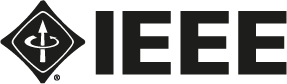
\includegraphics[bb= xlow ylow xhigh yhigh]{figs/myfigure.png}
%\caption{A simple figure.}
%\end{figure} 
\begin{thebibliography}{10}
\itemsep=1pt
\begin{small}

\bibitem{RK93}
	R.\ Alonso and H.\ F.\ Korth.
	\newblock Database System Issues in Nomadic Computing.
	\newblock Proc.\ ACM SIGMOD International Conference on
               Management of Data, 1993.
               
\bibitem{micali}
	M.\ Ben-Or, O.\ Goldreich, S.\ Goldwasser, J.\ Håstad, J.\ Kilian, S.\ Micali, and P.\ Rogaway.
	\newblock Everything Provable is Provable in Zero-Knowledge.
	\newblock {\em Advances in Cryptology — {CRYPTO}’ 88}.,
	Springer,
	1988.
	
\bibitem{cap12}
	E. Brewer. 
	\newblock CAP Twelve Years Later: How the ``Rules" Have Changed.
	\newblock {\em Computer}, vol. 45, no. 2, pp. 23-29, Feb. 2012.
	
\bibitem{fed}
	Board of Governors of the Federal Reserve System.
	\newblock {\em Money and Payments: The U.S.\ Dollar in the Age of Digital
Transformation}, Jan 2022.

\bibitem{jack}
	J.\ Byers.
	\newblock {\em Combating Front-running in the Blockchain Ecosystem}.
	\newblock Masters Thesis, Lehigh University, 2022.
	
\bibitem {flashboys}
	P.\ Daian, S.\ Goldfeder, T.\ Kell, Y.\ Li, X.\ Zhao, I.\ Bentov, L.\ Breidenbach, and A.\ Juels.
	\newblock Flash Boys 2.0: Frontrunning in Decentralized Exchanges, Miner Extractable Value, and Consensus Instability.
	\newblock {\em 2020 IEEE Symposium on Security and Privacy}

\bibitem{margo} 
J.\ Cheney and
               S.\ Chong,
               N.\ Foster,
               M.\ I.\ Seltzer,
               S.\ Vansummeren.  \newblock Provenance: a future history. \newblock {OOPSALA}, 2009.
               
\bibitem{dh76}
	W.\ Diffie and M.\ Hellman.
	\newblock New Directions in Cryptography.
	\newblock {\em IEEE Transactions on Information Theory}, 22:6, 1976.

\bibitem{Fanusie21}
Y.~J. Fanusie and E.~Jin.
\newblock China's digital currency.
\newblock {\em Technical report, Center for a New American Security}, 2021.

\bibitem{Knox}
	{\em Knox Networks Provides Feedback to the Federal Reserve on a Potential US Digital Dollar}, May 2022.
	\newblock https://medium.com/@knoxnetworks/knox-networks-provides-feedback-to-the-federal-reserve-on-a-potential-digital-dollar-fb7e77418fca


\bibitem{snow} H.\ F.\ Korth, N.\ M.\ Snow, and B.\ B.\ Fanuscu.
\newblock Provably Correct Financial Disclosures.
\newblock {\em In Preparation}. 2022.

\bibitem{levyPODC}
	E.\ Levy, H.\ F.\ Korth, and A. Silberschatz.
	\newblock A Theory of Relaxed Atomicity.
	\newblock Proc.\  1991 ACM Symposium on Principles of Distributed Computing (PODC).

\bibitem{StellarSOSP19}
	G.\ Losa, E.\  Gafni, and D.\ Mazi\`eres.
	\newblock Fast and secure global payments with {S}tellar.
	\newblock Proc.\ 27th ACM Symposium on Operating Systems Principles (SOSP),
	2019.
	

\bibitem{OM23} O.~Malekan.
                \newblock {\em Re-Architecting Trust: The curse of history and the crypto 
cure for money, markets, and platforms}. \newblock {Bookbaby, Pennsauken, NJ}, 2022.

\bibitem{SIG92}
	S.\ Mehrotra,
               R.\ Rastogi,
               Y.\ Breitbart,
               H.\ F.\ Korth, and
               A.\ Silberschatz.
               \newblock The Concurrency Control Problem in Multidatabases: Characteristics
               and Solutions.
               \newblock ACM SIGMOD International Conference on
               Management of Data, 1992.
               
\bibitem{Merkle87}
	R C. Merkle.
	\newblock A Digital Signature Based on a Conventional Encryption Function.
	\newblock Advances in Cryptology --- CRYPTO '87, Springer,
	1987.
	
\bibitem{Will21}
	W.\ Peracchio.
	\newblock {\em Design Considerations for Central Bank Digital Currencies}.
	\newblock Masters Thesis, Lehigh University, 2021.

\bibitem{DSC-BCDB}
A.~Silberschatz, H.~F. Korth, and S.~Sudarshan.
\newblock {\em Database System Concepts, 7th edition}, chapter 26: Blockchain
  Databases.
\newblock McGraw Hill Education, New York, NY, 2020.

\bibitem{max}
	M.\ Vezenov.
	\newblock {\em Accelerating zkSNARKs on Modern Architectures}.
	\newblock Masters Thesis, Lehigh University, 2022.
	
\bibitem{WB}
	World Bank.
	\newblock {\em Global Findex Database.}
	\newblock global.findex.worldbank.org
	               
\bibitem{w3c}
	 World-Wide Web Consortium.
	\newblock {\em Verifiable Credentials Data Model v1.1}, March 2022
	\newblock https://www.w3.org/TR/vc-data-model/
	
\bibitem{hotstuff}
	M.\ Yin, D.\ Malkhi, M.\ K.\ Reiter, G.\ G.\ Gueta, and I.\ Abraham.
	\newblock HotStuff: BFT Consensus with Linearity and Responsiveness
	\newblock Proc.\  2019 ACM Symposium on Principles of Distributed Computing (PODC).

\bibitem{Elmagarmid}
	A.\ Zhang and
               A.\ K. Elmagarmid.
               \newblock A Theory of Global Concurrency Control in Multidatabase Systems.
               \newblock {\em VLDB Journal} vol.\ 2 no.\ 3, 1993.
               
\bibitem{PipeZK}
 	Y.\ Zhang,
               S.\ Wang,
               X.\ Zhang,
               J.\ Dong,
               X.\ Mao,
               F.\ Long,
               C.\ Wang,
               D.\ Zhou,
               M.\ Gao, and
               G.  Sun.
	\newblock PipeZK: Accelerating Zero-Knowledge Proof with a Pipelined Architecture.
  	\newblock 48th {ACM/IEEE} Annual International Symposium on Computer Architecture,
               {ISCA} 2021.

\end{small}
\end{thebibliography}
\end{document}